%
\documentclass[12pt,border={0 0.5cm 0 .5cm}]{standalone}
%
\usepackage{tikz}
\usetikzlibrary{calc}
%
\tikzset{
  kosys/.pic={
	\draw[latex-latex] (0,1) --(0,0)node[sloped,pos=-0.2,rotate=90]{$y_{#1}$}--(1,0) node[sloped,pos=1.2]{$x_{#1}$};
  }
	}
%
\begin{document}
%
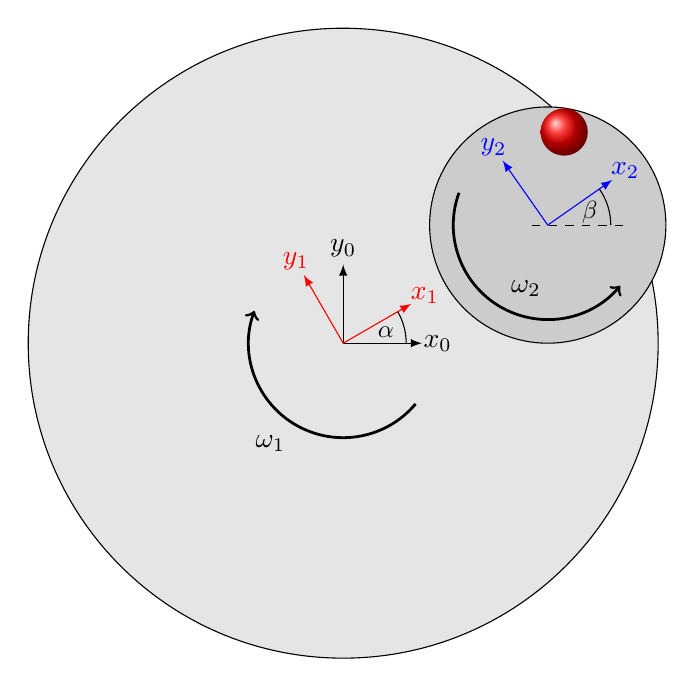
\begin{tikzpicture}
%
\def\R{4cm}
\def\r{1.5cm}
\def\rm{0.8cm}
\def\rb{0.3cm}
\def\alph{30}
\def\bet{35}
%
\coordinate(O)at(0,0);
\coordinate(A)at(\alph:\R-\r+0.5cm);
%
\draw[fill=gray!20] (O) circle (\R);
\draw[fill=gray!40] (A) circle (\r);
%
\shade[ball color=red] ($(A)+(80:\r-\rb)$) circle (\rb);
%
\pic[scale=1] at (O) {kosys=0};
\pic[scale=1,color=red,rotate=\alph] at (O) {kosys=1};
\pic[scale=1,rotate=\bet, color=blue] at (A) {kosys=2};
%
\draw[]($(O)+(0:\rm)$) arc(0:\alph:\rm);
\node[scale=0.9] at ($(O)+(0.5*\alph:0.7*\rm)$){$\alpha$};
%
\draw[dashed] ($(A)+(-0.2,0)$) --+(1.2,0);
\draw[]($(A)+(0:\rm)$) arc(0:\bet:\rm);
\node[scale=0.9] at ($(A)+(0.5*\bet:0.7*\rm)$){$\beta$};
%
\draw[line width=1pt,<-] ($(O)+(160:1.2)$) arc (160:320:1.2)node[pos=0.5,anchor=north east]{$\omega_1$};
\draw[line width=1pt,->] ($(A)+(160:1.2)$) arc (160:320:1.2)node[pos=0.5,anchor=south west]{$\omega_2$};
%
\end{tikzpicture}
%
\end{document}